% Options for packages loaded elsewhere
\PassOptionsToPackage{unicode}{hyperref}
\PassOptionsToPackage{hyphens}{url}
%
\documentclass[
  ignorenonframetext,
]{beamer}
\usepackage{pgfpages}
\setbeamertemplate{caption}[numbered]
\setbeamertemplate{caption label separator}{: }
\setbeamercolor{caption name}{fg=normal text.fg}
\beamertemplatenavigationsymbolsempty
% Prevent slide breaks in the middle of a paragraph
\widowpenalties 1 10000
\raggedbottom
\setbeamertemplate{part page}{
  \centering
  \begin{beamercolorbox}[sep=16pt,center]{part title}
    \usebeamerfont{part title}\insertpart\par
  \end{beamercolorbox}
}
\setbeamertemplate{section page}{
  \centering
  \begin{beamercolorbox}[sep=12pt,center]{part title}
    \usebeamerfont{section title}\insertsection\par
  \end{beamercolorbox}
}
\setbeamertemplate{subsection page}{
  \centering
  \begin{beamercolorbox}[sep=8pt,center]{part title}
    \usebeamerfont{subsection title}\insertsubsection\par
  \end{beamercolorbox}
}
\AtBeginPart{
  \frame{\partpage}
}
\AtBeginSection{
  \ifbibliography
  \else
    \frame{\sectionpage}
  \fi
}
\AtBeginSubsection{
  \frame{\subsectionpage}
}
\usepackage{amsmath,amssymb}
\usepackage{lmodern}
\usepackage{iftex}
\ifPDFTeX
  \usepackage[T1]{fontenc}
  \usepackage[utf8]{inputenc}
  \usepackage{textcomp} % provide euro and other symbols
\else % if luatex or xetex
  \usepackage{unicode-math}
  \defaultfontfeatures{Scale=MatchLowercase}
  \defaultfontfeatures[\rmfamily]{Ligatures=TeX,Scale=1}
\fi
\usecolortheme{dolphin}
% Use upquote if available, for straight quotes in verbatim environments
\IfFileExists{upquote.sty}{\usepackage{upquote}}{}
\IfFileExists{microtype.sty}{% use microtype if available
  \usepackage[]{microtype}
  \UseMicrotypeSet[protrusion]{basicmath} % disable protrusion for tt fonts
}{}
\makeatletter
\@ifundefined{KOMAClassName}{% if non-KOMA class
  \IfFileExists{parskip.sty}{%
    \usepackage{parskip}
  }{% else
    \setlength{\parindent}{0pt}
    \setlength{\parskip}{6pt plus 2pt minus 1pt}}
}{% if KOMA class
  \KOMAoptions{parskip=half}}
\makeatother
\usepackage{xcolor}
\newif\ifbibliography
\usepackage{color}
\usepackage{fancyvrb}
\newcommand{\VerbBar}{|}
\newcommand{\VERB}{\Verb[commandchars=\\\{\}]}
\DefineVerbatimEnvironment{Highlighting}{Verbatim}{commandchars=\\\{\}}
% Add ',fontsize=\small' for more characters per line
\usepackage{framed}
\definecolor{shadecolor}{RGB}{248,248,248}
\newenvironment{Shaded}{\begin{snugshade}}{\end{snugshade}}
\newcommand{\AlertTok}[1]{\textcolor[rgb]{0.94,0.16,0.16}{#1}}
\newcommand{\AnnotationTok}[1]{\textcolor[rgb]{0.56,0.35,0.01}{\textbf{\textit{#1}}}}
\newcommand{\AttributeTok}[1]{\textcolor[rgb]{0.77,0.63,0.00}{#1}}
\newcommand{\BaseNTok}[1]{\textcolor[rgb]{0.00,0.00,0.81}{#1}}
\newcommand{\BuiltInTok}[1]{#1}
\newcommand{\CharTok}[1]{\textcolor[rgb]{0.31,0.60,0.02}{#1}}
\newcommand{\CommentTok}[1]{\textcolor[rgb]{0.56,0.35,0.01}{\textit{#1}}}
\newcommand{\CommentVarTok}[1]{\textcolor[rgb]{0.56,0.35,0.01}{\textbf{\textit{#1}}}}
\newcommand{\ConstantTok}[1]{\textcolor[rgb]{0.00,0.00,0.00}{#1}}
\newcommand{\ControlFlowTok}[1]{\textcolor[rgb]{0.13,0.29,0.53}{\textbf{#1}}}
\newcommand{\DataTypeTok}[1]{\textcolor[rgb]{0.13,0.29,0.53}{#1}}
\newcommand{\DecValTok}[1]{\textcolor[rgb]{0.00,0.00,0.81}{#1}}
\newcommand{\DocumentationTok}[1]{\textcolor[rgb]{0.56,0.35,0.01}{\textbf{\textit{#1}}}}
\newcommand{\ErrorTok}[1]{\textcolor[rgb]{0.64,0.00,0.00}{\textbf{#1}}}
\newcommand{\ExtensionTok}[1]{#1}
\newcommand{\FloatTok}[1]{\textcolor[rgb]{0.00,0.00,0.81}{#1}}
\newcommand{\FunctionTok}[1]{\textcolor[rgb]{0.00,0.00,0.00}{#1}}
\newcommand{\ImportTok}[1]{#1}
\newcommand{\InformationTok}[1]{\textcolor[rgb]{0.56,0.35,0.01}{\textbf{\textit{#1}}}}
\newcommand{\KeywordTok}[1]{\textcolor[rgb]{0.13,0.29,0.53}{\textbf{#1}}}
\newcommand{\NormalTok}[1]{#1}
\newcommand{\OperatorTok}[1]{\textcolor[rgb]{0.81,0.36,0.00}{\textbf{#1}}}
\newcommand{\OtherTok}[1]{\textcolor[rgb]{0.56,0.35,0.01}{#1}}
\newcommand{\PreprocessorTok}[1]{\textcolor[rgb]{0.56,0.35,0.01}{\textit{#1}}}
\newcommand{\RegionMarkerTok}[1]{#1}
\newcommand{\SpecialCharTok}[1]{\textcolor[rgb]{0.00,0.00,0.00}{#1}}
\newcommand{\SpecialStringTok}[1]{\textcolor[rgb]{0.31,0.60,0.02}{#1}}
\newcommand{\StringTok}[1]{\textcolor[rgb]{0.31,0.60,0.02}{#1}}
\newcommand{\VariableTok}[1]{\textcolor[rgb]{0.00,0.00,0.00}{#1}}
\newcommand{\VerbatimStringTok}[1]{\textcolor[rgb]{0.31,0.60,0.02}{#1}}
\newcommand{\WarningTok}[1]{\textcolor[rgb]{0.56,0.35,0.01}{\textbf{\textit{#1}}}}
\usepackage{longtable,booktabs,array}
\usepackage{calc} % for calculating minipage widths
\usepackage{caption}
% Make caption package work with longtable
\makeatletter
\def\fnum@table{\tablename~\thetable}
\makeatother
\usepackage{graphicx}
\makeatletter
\def\maxwidth{\ifdim\Gin@nat@width>\linewidth\linewidth\else\Gin@nat@width\fi}
\def\maxheight{\ifdim\Gin@nat@height>\textheight\textheight\else\Gin@nat@height\fi}
\makeatother
% Scale images if necessary, so that they will not overflow the page
% margins by default, and it is still possible to overwrite the defaults
% using explicit options in \includegraphics[width, height, ...]{}
\setkeys{Gin}{width=\maxwidth,height=\maxheight,keepaspectratio}
% Set default figure placement to htbp
\makeatletter
\def\fps@figure{htbp}
\makeatother
\setlength{\emergencystretch}{3em} % prevent overfull lines
\providecommand{\tightlist}{%
  \setlength{\itemsep}{0pt}\setlength{\parskip}{0pt}}
\setcounter{secnumdepth}{-\maxdimen} % remove section numbering
\ifLuaTeX
  \usepackage{selnolig}  % disable illegal ligatures
\fi
\IfFileExists{bookmark.sty}{\usepackage{bookmark}}{\usepackage{hyperref}}
\IfFileExists{xurl.sty}{\usepackage{xurl}}{} % add URL line breaks if available
\urlstyle{same} % disable monospaced font for URLs
\hypersetup{
  hidelinks,
  pdfcreator={LaTeX via pandoc}}

\title{Evaluating and Extending Three-Arm\\
Study in the Treatment of Superficial\\
Bladder Cancer\\
\strut \\
P8108 Final Project, Fall 2022\\}
\author{Yunyi Jiang, Xiao Ma, Waveley Qiu,\\
Xuehan Yan, Congyang Xie\\}
\date{2022-12-05}

\begin{document}
\frame{\titlepage}

\hypertarget{background}{%
\section{Background}\label{background}}

\begin{frame}{Superficial Bladder Cancer}
\protect\hypertarget{superficial-bladder-cancer}{}
\begin{itemize}
\tightlist
\item
  Also known as Stage 1 bladder cancer
\item
  Common diagnosis (75\% of bladder cancer cases\(^1\)) and rarely
  life-threatening on it own.
\item
  Thought to arise due to urinary issues\(^1\) or through
  ``abnormalities of tryptophan metabolism''\(^2\)
\item
  Particular interest in preventing recurrence of disease

  \begin{itemize}
  \tightlist
  \item
    Natural history study conducted in Sweden saw that ``death was
    directly related to tumor grade, number of tumors, and volume of
    recurrences.''\(^3\)
  \end{itemize}
\end{itemize}
\end{frame}

\begin{frame}{Pyridoxine and Thiotepa}
\protect\hypertarget{pyridoxine-and-thiotepa}{}
\begin{itemize}
\tightlist
\item
  \emph{Pyridoxine} (vitamin \(B_6\)) thought to reduce ``abnormalities
  of tryptophan metabolism''
\item
  \emph{Thiotepa} has been the standard of care for the treatment of
  superficial bladder cancers.
\item
  Effects of these two therapies compared in randomized clinical trial
  conducted by Byar and Blackard in 1977
\end{itemize}
\end{frame}

\begin{frame}{Byar and Blackard (1977)}
\protect\hypertarget{byar-and-blackard-1977}{}
\begin{itemize}
\tightlist
\item
  Primary clinical interest: prevent and reduce recurrence of Stage 1
  bladder cancer.
\item
  Event time agnostic analysis conducted included comparing overall
  rates and percentages of occurrence between groups

  \begin{itemize}
  \tightlist
  \item
    Pairwise difference detected in rate of recurrence between thiotepa
    and placebo, and thiotepa and pyridoxine
  \item
    No other differences in event incidence between groups detected
  \end{itemize}
\item
  Survival analysis conducted involved the construction of life-table
  estimates.

  \begin{itemize}
  \tightlist
  \item
    Life-table analysis indicate that the time to first recurrence was
    significantly different between pyridoxine and placebo groups.
  \item
    Analysis restricted to subjects who experienced recurrence after at
    least 10 months of follow-up
  \end{itemize}
\end{itemize}
\end{frame}

\hypertarget{proposed-project}{%
\section{Proposed Project}\label{proposed-project}}

\begin{frame}{Motivation}
\protect\hypertarget{motivation}{}
\begin{itemize}
\tightlist
\item
  Research ought to be reproducible, especially if data are open-source
\item
  Different models may be more informative than the actuarial curves
  constructed
\end{itemize}
\end{frame}

\begin{frame}{Analysis Plan}
\protect\hypertarget{analysis-plan}{}
\begin{enumerate}
\tightlist
\item
  Reproduce analysis conducted in original study to see if results can
  be replicated
\item
  Construct models that differ from original study to see if they can be
  more informative
\end{enumerate}

\begin{itemize}
\tightlist
\item
  Non-parametric: KM
\item
  Semi-parametric: Cox Proportional Hazards Model
\item
  Parametric: Weibull and Exponential Models
\end{itemize}
\end{frame}

\begin{frame}[fragile]{Exploratory Data Analysis}
\protect\hypertarget{exploratory-data-analysis}{}
\begin{Shaded}
\begin{Highlighting}[]
\FunctionTok{ggplot}\NormalTok{(}\AttributeTok{data =}\NormalTok{ p1, }\FunctionTok{aes}\NormalTok{(}\AttributeTok{x =}\NormalTok{ treatment, }\AttributeTok{y =}\NormalTok{ n, }\AttributeTok{fill=}\FunctionTok{factor}\NormalTok{(recurrence))) }\SpecialCharTok{+} \FunctionTok{geom\_bar}\NormalTok{(}\AttributeTok{stat=}\StringTok{"identity"}\NormalTok{,}\AttributeTok{color =} \StringTok{"black"}\NormalTok{) }\SpecialCharTok{+} \FunctionTok{geom\_text}\NormalTok{(}\FunctionTok{aes}\NormalTok{(}\AttributeTok{label =}\NormalTok{ n),}\AttributeTok{color =} \StringTok{"black"}\NormalTok{,}\AttributeTok{hjust =} \FloatTok{0.5}\NormalTok{,}\AttributeTok{vjust =} \DecValTok{3}\NormalTok{,}\AttributeTok{size =} \DecValTok{3}\NormalTok{,}\AttributeTok{position =} \StringTok{"stack"}\NormalTok{) }\SpecialCharTok{+} \FunctionTok{labs}\NormalTok{(}\AttributeTok{title =} \StringTok{"Distribution of patients for Each Treatment and Recurrence "}\NormalTok{, }\AttributeTok{x =} \StringTok{"Treatment"}\NormalTok{, }\AttributeTok{y =}\StringTok{"Number of Patients"}\NormalTok{) }\SpecialCharTok{+} \FunctionTok{guides}\NormalTok{(}\AttributeTok{fill =} \FunctionTok{guide\_legend}\NormalTok{(}\AttributeTok{title =} \StringTok{"Recurrence"}\NormalTok{)) }\SpecialCharTok{+} \FunctionTok{scale\_fill\_manual}\NormalTok{(}\AttributeTok{values =} \FunctionTok{c}\NormalTok{(}\StringTok{\textquotesingle{}light blue\textquotesingle{}}\NormalTok{,}\StringTok{\textquotesingle{}orchid\textquotesingle{}}\NormalTok{))}
\end{Highlighting}
\end{Shaded}

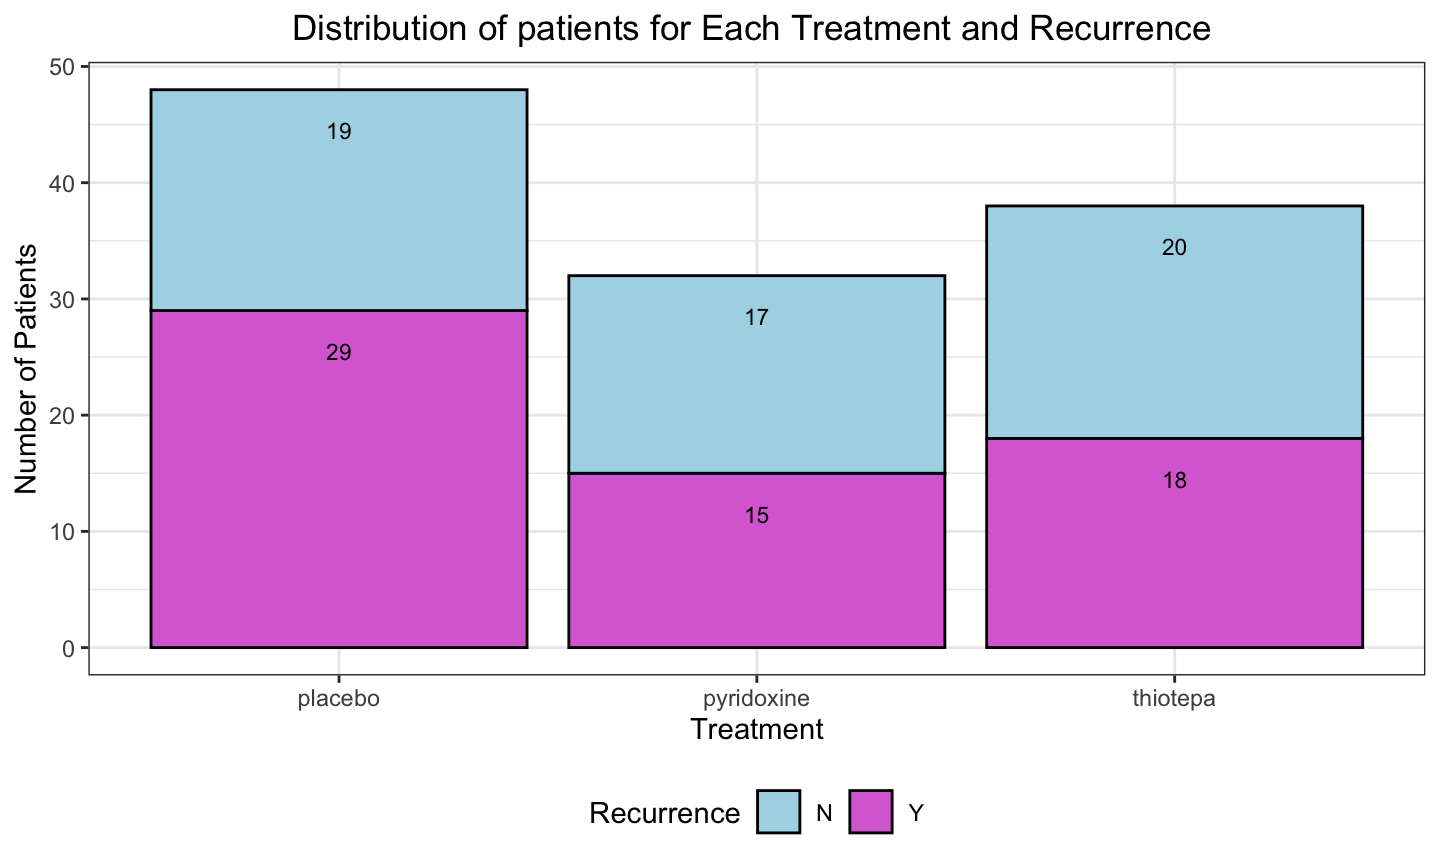
\includegraphics{presentation_files/figure-beamer/unnamed-chunk-4-1.pdf}
*Number of patients in the three treatment groups are shown. Patients
were assigned at random with equal probability but numbers in the three
treatment groups are not equal.
\end{frame}

\begin{frame}[fragile]{Distribution of Patient Final Status over
Different Treatment}
\protect\hypertarget{distribution-of-patient-final-status-over-different-treatment}{}
\begin{Shaded}
\begin{Highlighting}[]
\NormalTok{final\_status }\OtherTok{=}\NormalTok{ bladder }\SpecialCharTok{\%\textgreater{}\%}  
  \FunctionTok{select}\NormalTok{(id,treatment,recur,status) }\SpecialCharTok{\%\textgreater{}\%} 
  \FunctionTok{group\_by}\NormalTok{(treatment,status) }\SpecialCharTok{\%\textgreater{}\%} \FunctionTok{summarise}\NormalTok{(}\AttributeTok{n =} \FunctionTok{n}\NormalTok{())}
\end{Highlighting}
\end{Shaded}

\begin{verbatim}
## `summarise()` has grouped output by 'treatment'. You can override using the `.groups` argument.
\end{verbatim}

\begin{Shaded}
\begin{Highlighting}[]
\NormalTok{p2 }\OtherTok{=} \FunctionTok{data.frame}\NormalTok{(final\_status)}

\FunctionTok{ggplot}\NormalTok{(}\AttributeTok{data=}\NormalTok{p2, }\FunctionTok{aes}\NormalTok{(}\AttributeTok{x=}\FunctionTok{as.factor}\NormalTok{(status), }\AttributeTok{y=}\NormalTok{ n,}\AttributeTok{fill=}\FunctionTok{as.factor}\NormalTok{(status))) }\SpecialCharTok{+} \FunctionTok{geom\_bar}\NormalTok{(}\AttributeTok{stat=}\StringTok{"identity"}\NormalTok{, }\AttributeTok{position=}\FunctionTok{position\_dodge}\NormalTok{())}\SpecialCharTok{+}\FunctionTok{geom\_text}\NormalTok{(}\FunctionTok{aes}\NormalTok{(}\AttributeTok{label =}\NormalTok{ n),}\AttributeTok{color =} \StringTok{"white"}\NormalTok{,}\AttributeTok{hjust=}\FloatTok{0.2}\NormalTok{,}\AttributeTok{vjust=}\FloatTok{1.5}\NormalTok{,}\AttributeTok{size=}\DecValTok{3}\NormalTok{,}\AttributeTok{position =} \FunctionTok{position\_dodge}\NormalTok{(}\FloatTok{0.9}\NormalTok{))}\SpecialCharTok{+}\FunctionTok{facet\_grid}\NormalTok{(. }\SpecialCharTok{\textasciitilde{}}\NormalTok{ treatment) }\SpecialCharTok{+} \FunctionTok{labs}\NormalTok{(}\AttributeTok{title=}\StringTok{"Distribution of Patient Final Status over Different Treatment"}\NormalTok{, }\AttributeTok{x =} \StringTok{"Status"}\NormalTok{, }\AttributeTok{y =} \StringTok{"Counts"}\NormalTok{, }\AttributeTok{fill =} \StringTok{"Status"}\NormalTok{)}\SpecialCharTok{+} \FunctionTok{scale\_fill\_discrete}\NormalTok{(}\AttributeTok{labels=}\FunctionTok{c}\NormalTok{(}\StringTok{\textquotesingle{}Censored\textquotesingle{}}\NormalTok{, }\StringTok{\textquotesingle{}Recurrence\textquotesingle{}}\NormalTok{,}\StringTok{\textquotesingle{}Death of Bladder\textquotesingle{}}\NormalTok{, }\StringTok{\textquotesingle{}Death Other Cause\textquotesingle{}}\NormalTok{))}
\end{Highlighting}
\end{Shaded}

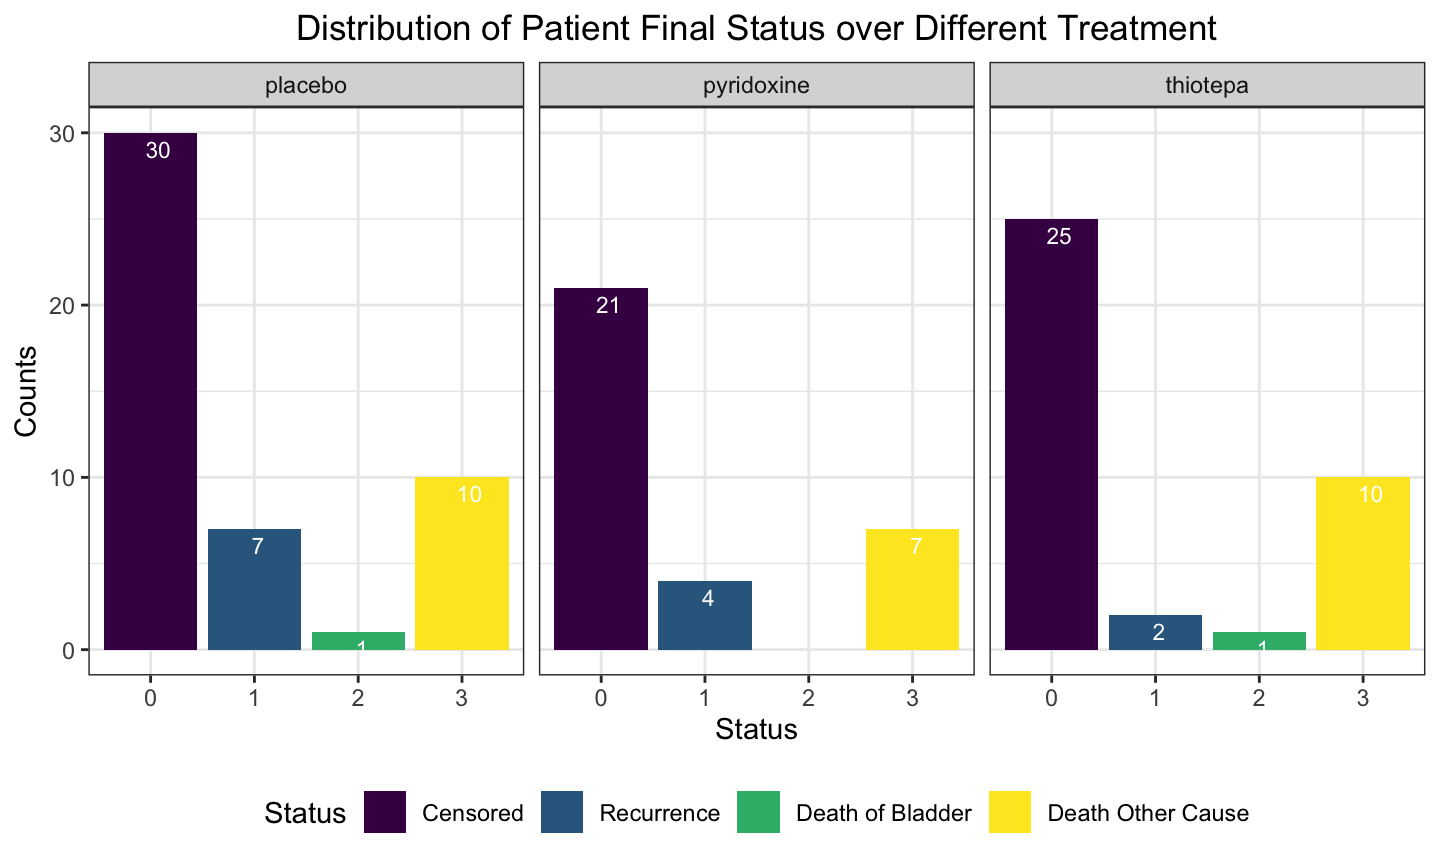
\includegraphics{presentation_files/figure-beamer/unnamed-chunk-5-1.pdf}
\end{frame}

\begin{frame}[fragile]{Distribution of Recurrences Patients Final Status
of over Treatment}
\protect\hypertarget{distribution-of-recurrences-patients-final-status-of-over-treatment}{}
\begin{Shaded}
\begin{Highlighting}[]
\NormalTok{p3 }\OtherTok{=}\NormalTok{ bladder }\SpecialCharTok{\%\textgreater{}\%} 
  \FunctionTok{filter}\NormalTok{(recur }\SpecialCharTok{\textgreater{}} \DecValTok{0}\NormalTok{) }\SpecialCharTok{\%\textgreater{}\%} 
  \FunctionTok{select}\NormalTok{(id,treatment,recur,status) }\SpecialCharTok{\%\textgreater{}\%} 
  \FunctionTok{group\_by}\NormalTok{(treatment,status) }\SpecialCharTok{\%\textgreater{}\%} \FunctionTok{summarise}\NormalTok{(}\AttributeTok{n =} \FunctionTok{n}\NormalTok{())}
\end{Highlighting}
\end{Shaded}

\begin{verbatim}
## `summarise()` has grouped output by 'treatment'. You can override using the `.groups` argument.
\end{verbatim}

\begin{Shaded}
\begin{Highlighting}[]
\FunctionTok{ggplot}\NormalTok{(}\AttributeTok{data=}\NormalTok{p3, }\FunctionTok{aes}\NormalTok{(}\AttributeTok{x =} \FunctionTok{as.factor}\NormalTok{(status), }\AttributeTok{y =}\NormalTok{ n,}\AttributeTok{fill =} \FunctionTok{as.factor}\NormalTok{(status))) }\SpecialCharTok{+} \FunctionTok{geom\_bar}\NormalTok{(}\AttributeTok{stat =} \StringTok{"identity"}\NormalTok{, }\AttributeTok{position =} \FunctionTok{position\_dodge}\NormalTok{()) }\SpecialCharTok{+} \FunctionTok{geom\_text}\NormalTok{(}\FunctionTok{aes}\NormalTok{(}\AttributeTok{label =}\NormalTok{ n),}\AttributeTok{color =} \StringTok{"white"}\NormalTok{,}\AttributeTok{hjust =} \FloatTok{0.2}\NormalTok{,}\AttributeTok{vjust=}\FloatTok{1.5}\NormalTok{,}\AttributeTok{size =} \DecValTok{3}\NormalTok{,}\AttributeTok{position =} \FunctionTok{position\_dodge}\NormalTok{(}\FloatTok{0.9}\NormalTok{)) }\SpecialCharTok{+} \FunctionTok{facet\_grid}\NormalTok{(. }\SpecialCharTok{\textasciitilde{}}\NormalTok{ treatment) }\SpecialCharTok{+} 
\FunctionTok{labs}\NormalTok{(}\AttributeTok{title =} \StringTok{"Distrubition of Final Status of Recurrence Patients"}\NormalTok{, }\AttributeTok{x =} \StringTok{"status"}\NormalTok{, }\AttributeTok{y =} \StringTok{"counts"}\NormalTok{, }\AttributeTok{fill =} \StringTok{"status"}\NormalTok{)}\SpecialCharTok{+} \FunctionTok{scale\_fill\_discrete}\NormalTok{(}\AttributeTok{labels=}\FunctionTok{c}\NormalTok{(}\StringTok{\textquotesingle{}Censored\textquotesingle{}}\NormalTok{, }\StringTok{\textquotesingle{}Recurrence\textquotesingle{}}\NormalTok{,}\StringTok{\textquotesingle{}Death of Bladder\textquotesingle{}}\NormalTok{, }\StringTok{\textquotesingle{}Death Other Cause\textquotesingle{}}\NormalTok{))}
\end{Highlighting}
\end{Shaded}

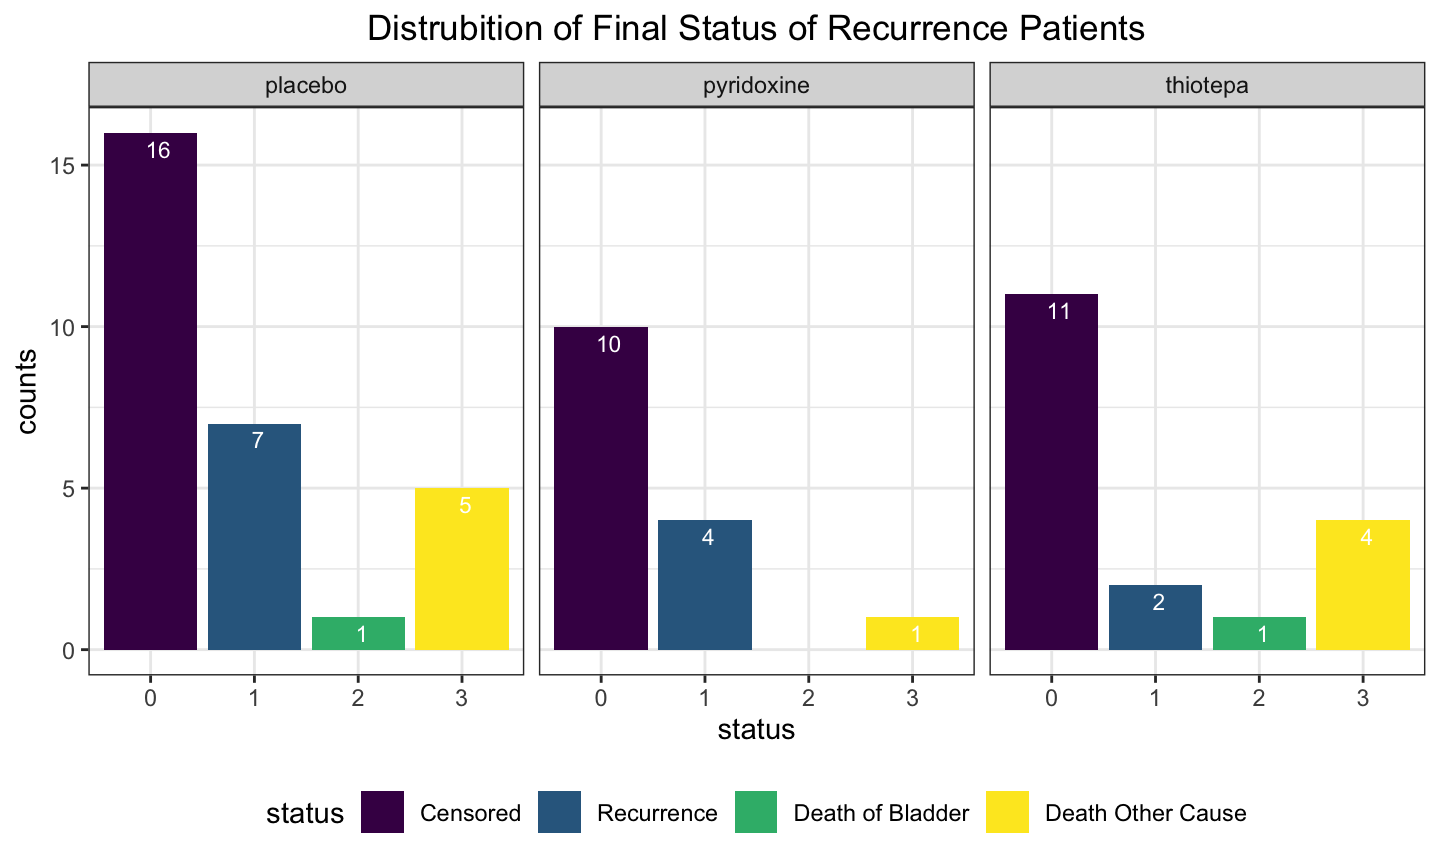
\includegraphics{presentation_files/figure-beamer/unnamed-chunk-6-1.pdf}
\end{frame}

\begin{frame}[fragile]{Distribution of Number of tumors and The Largest
Initial Tumor SIze}
\protect\hypertarget{distribution-of-number-of-tumors-and-the-largest-initial-tumor-size}{}
\begin{Shaded}
\begin{Highlighting}[]
\NormalTok{p4 }\OtherTok{=}\NormalTok{  bladder }\SpecialCharTok{\%\textgreater{}\%} \FunctionTok{select}\NormalTok{(id,treatment,number,size) }\SpecialCharTok{\%\textgreater{}\%} \FunctionTok{group\_by}\NormalTok{(treatment)}

\FunctionTok{ggplot}\NormalTok{(p4, }\FunctionTok{aes}\NormalTok{(}\AttributeTok{x =}\NormalTok{ number, }\AttributeTok{y =}\NormalTok{ size, }\AttributeTok{color =}\NormalTok{ treatment)) }\SpecialCharTok{+} 
  \FunctionTok{geom\_point}\NormalTok{(}\AttributeTok{alpha =}\NormalTok{ .}\DecValTok{5}\NormalTok{,}\AttributeTok{position =} \StringTok{"jitter"}\NormalTok{) }\SpecialCharTok{+}
  \FunctionTok{xlim}\NormalTok{(}\DecValTok{1}\NormalTok{,}\DecValTok{8}\NormalTok{) }\SpecialCharTok{+}
  \FunctionTok{ylim}\NormalTok{(}\DecValTok{1}\NormalTok{,}\DecValTok{8}\NormalTok{) }\SpecialCharTok{+}
  \FunctionTok{facet\_grid}\NormalTok{(. }\SpecialCharTok{\textasciitilde{}}\NormalTok{ treatment)}
\end{Highlighting}
\end{Shaded}

\begin{verbatim}
## Warning: Removed 71 rows containing missing values (geom_point).
\end{verbatim}

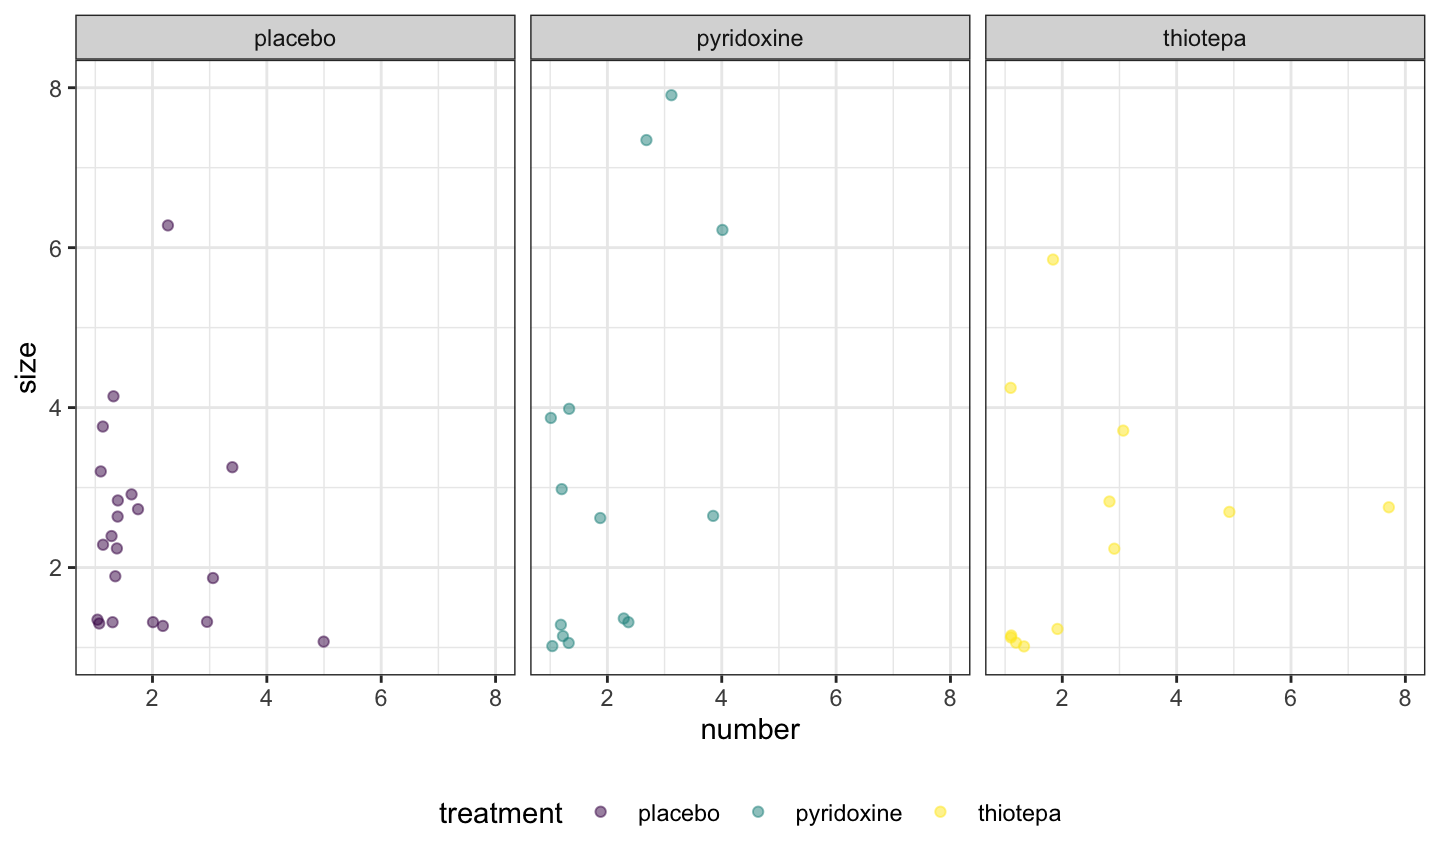
\includegraphics{presentation_files/figure-beamer/unnamed-chunk-7-1.pdf}
\end{frame}

\begin{frame}[fragile]{Examine whether number of tumors/size of tumors
has something to do with number of recurrences}
\protect\hypertarget{examine-whether-number-of-tumorssize-of-tumors-has-something-to-do-with-number-of-recurrences}{}
\begin{Shaded}
\begin{Highlighting}[]
\NormalTok{p5 }\OtherTok{=}\NormalTok{ bladder }\SpecialCharTok{\%\textgreater{}\%} \FunctionTok{filter}\NormalTok{(recur }\SpecialCharTok{!=} \DecValTok{0}\NormalTok{) }\SpecialCharTok{\%\textgreater{}\%} 
     \FunctionTok{group\_by}\NormalTok{(id,treatment,recur,status,number,size) }\SpecialCharTok{\%\textgreater{}\%} \FunctionTok{summarise}\NormalTok{(}\AttributeTok{n =} \FunctionTok{n}\NormalTok{())}
\end{Highlighting}
\end{Shaded}

\begin{verbatim}
## `summarise()` has grouped output by 'id', 'treatment', 'recur', 'status', 'number'. You can override using the `.groups` argument.
\end{verbatim}

\begin{Shaded}
\begin{Highlighting}[]
\FunctionTok{ggplot}\NormalTok{(p5, }\FunctionTok{aes}\NormalTok{(}\AttributeTok{x =}\NormalTok{ number, }\AttributeTok{y =}\NormalTok{ size, }\AttributeTok{color =}\NormalTok{ recur)) }\SpecialCharTok{+} 
  \FunctionTok{geom\_point}\NormalTok{(}\AttributeTok{alpha =}\NormalTok{ .}\DecValTok{5}\NormalTok{, }\AttributeTok{position =} \StringTok{"jitter"}\NormalTok{) }\SpecialCharTok{+} 
  \FunctionTok{facet\_grid}\NormalTok{(. }\SpecialCharTok{\textasciitilde{}}\NormalTok{ treatment)}
\end{Highlighting}
\end{Shaded}

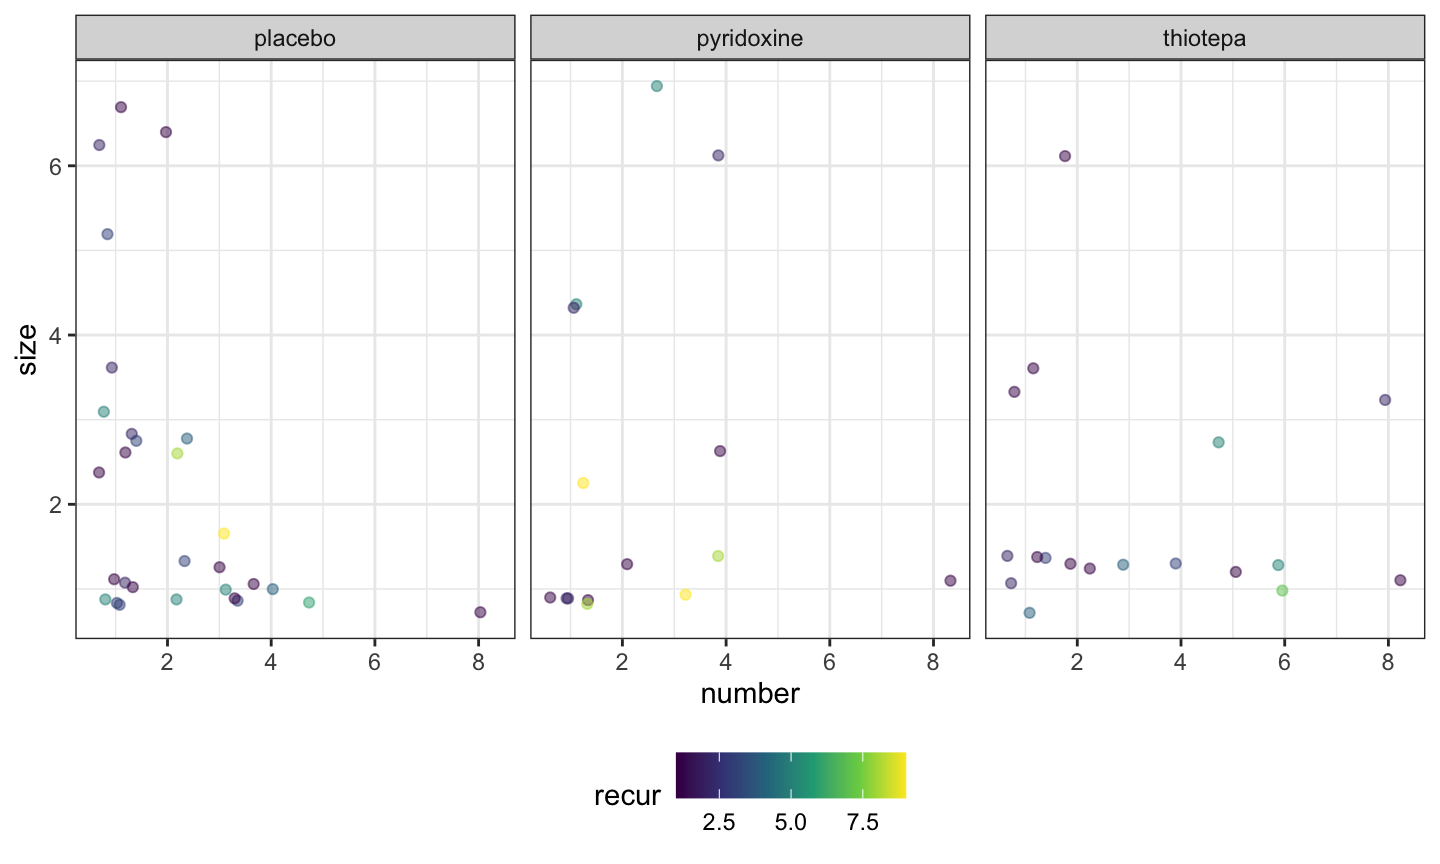
\includegraphics{presentation_files/figure-beamer/unnamed-chunk-8-1.pdf}
\end{frame}

\begin{frame}[fragile]{Initial Tumor Size and Number of Tumor with Final
Status}
\protect\hypertarget{initial-tumor-size-and-number-of-tumor-with-final-status}{}
\begin{Shaded}
\begin{Highlighting}[]
\NormalTok{p6 }\OtherTok{=}\NormalTok{ bladder }\SpecialCharTok{\%\textgreater{}\%} \FunctionTok{group\_by}\NormalTok{(id,treatment,status,size,number) }\SpecialCharTok{\%\textgreater{}\%} \FunctionTok{summarise}\NormalTok{(}\AttributeTok{n =} \FunctionTok{n}\NormalTok{())}
\end{Highlighting}
\end{Shaded}

\begin{verbatim}
## `summarise()` has grouped output by 'id', 'treatment', 'status', 'size'. You can override using the `.groups` argument.
\end{verbatim}

\begin{Shaded}
\begin{Highlighting}[]
\FunctionTok{ggplot}\NormalTok{(p6, }\FunctionTok{aes}\NormalTok{(}\AttributeTok{x =}\NormalTok{ number, }\AttributeTok{y =}\NormalTok{ size, }\AttributeTok{color =} \FunctionTok{factor}\NormalTok{(status))) }\SpecialCharTok{+} 
  \FunctionTok{geom\_point}\NormalTok{(}\AttributeTok{alpha =}\NormalTok{ .}\DecValTok{5}\NormalTok{, }\AttributeTok{position =} \StringTok{"jitter"}\NormalTok{) }\SpecialCharTok{+} 
  \FunctionTok{facet\_grid}\NormalTok{(. }\SpecialCharTok{\textasciitilde{}}\NormalTok{ treatment)}
\end{Highlighting}
\end{Shaded}

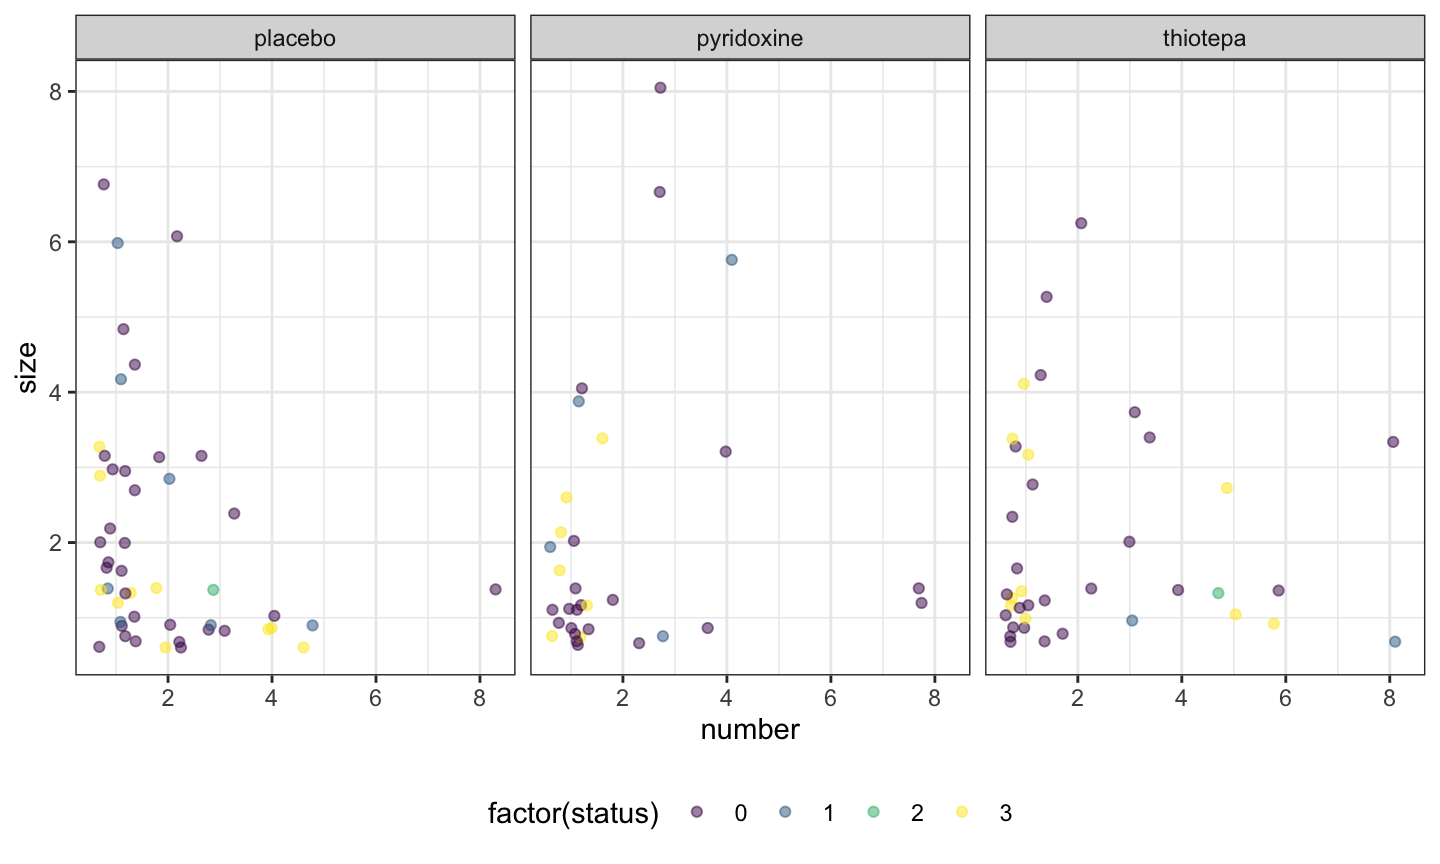
\includegraphics{presentation_files/figure-beamer/unnamed-chunk-9-1.pdf}
\end{frame}

\begin{frame}[fragile]{Exploratory Data Analysis}
\protect\hypertarget{exploratory-data-analysis-1}{}
\begin{longtable}[]{@{}
  >{\raggedleft\arraybackslash}p{(\columnwidth - 20\tabcolsep) * \real{0.0448}}
  >{\raggedright\arraybackslash}p{(\columnwidth - 20\tabcolsep) * \real{0.1493}}
  >{\raggedleft\arraybackslash}p{(\columnwidth - 20\tabcolsep) * \real{0.1045}}
  >{\raggedleft\arraybackslash}p{(\columnwidth - 20\tabcolsep) * \real{0.0746}}
  >{\raggedleft\arraybackslash}p{(\columnwidth - 20\tabcolsep) * \real{0.0896}}
  >{\raggedleft\arraybackslash}p{(\columnwidth - 20\tabcolsep) * \real{0.0896}}
  >{\raggedleft\arraybackslash}p{(\columnwidth - 20\tabcolsep) * \real{0.0746}}
  >{\raggedleft\arraybackslash}p{(\columnwidth - 20\tabcolsep) * \real{0.1045}}
  >{\raggedright\arraybackslash}p{(\columnwidth - 20\tabcolsep) * \real{0.1045}}
  >{\raggedright\arraybackslash}p{(\columnwidth - 20\tabcolsep) * \real{0.0896}}
  >{\raggedleft\arraybackslash}p{(\columnwidth - 20\tabcolsep) * \real{0.0746}}@{}}
\toprule()
\begin{minipage}[b]{\linewidth}\raggedleft
id
\end{minipage} & \begin{minipage}[b]{\linewidth}\raggedright
treatment
\end{minipage} & \begin{minipage}[b]{\linewidth}\raggedleft
number
\end{minipage} & \begin{minipage}[b]{\linewidth}\raggedleft
size
\end{minipage} & \begin{minipage}[b]{\linewidth}\raggedleft
recur
\end{minipage} & \begin{minipage}[b]{\linewidth}\raggedleft
start
\end{minipage} & \begin{minipage}[b]{\linewidth}\raggedleft
stop
\end{minipage} & \begin{minipage}[b]{\linewidth}\raggedleft
status
\end{minipage} & \begin{minipage}[b]{\linewidth}\raggedright
rtumor
\end{minipage} & \begin{minipage}[b]{\linewidth}\raggedright
rsize
\end{minipage} & \begin{minipage}[b]{\linewidth}\raggedleft
enum
\end{minipage} \\
\midrule()
\endhead
1 & placebo & 1 & 1 & 0 & 0 & 0 & 3 & . & . & 1 \\
2 & placebo & 1 & 3 & 0 & 0 & 1 & 3 & . & . & 1 \\
3 & placebo & 2 & 1 & 0 & 0 & 4 & 0 & . & . & 1 \\
4 & placebo & 1 & 1 & 0 & 0 & 7 & 0 & . & . & 1 \\
5 & placebo & 5 & 1 & 0 & 0 & 10 & 3 & . & . & 1 \\
6 & placebo & 4 & 1 & 1 & 0 & 6 & 1 & 1 & 1 & 1 \\
\bottomrule()
\end{longtable}

\begin{itemize}
\tightlist
\item
  \texttt{id}: Patient id
\item
  \texttt{treatment}: Placebo, pyridoxine (vitamin B6), or thiotepa
\item
  \texttt{recur}: Number of recurrences
\item
  \texttt{start}, \texttt{stop}: The start and end time of each time
  interval
\item
  \texttt{status}: End of interval code, 0=censored, 1=recurrence,
  2=death from bladder disease, 3=death from other/unknown cause
\end{itemize}
\end{frame}

\hypertarget{reproduction-analysis}{%
\section{Reproduction Analysis}\label{reproduction-analysis}}

\begin{frame}{}
\protect\hypertarget{section}{}
\begin{longtable}[]{@{}lrrr@{}}
\toprule()
name & Placebo & Pyridoxine & Thiotepa \\
\midrule()
\endhead
Evaluable Patients & 48.00 & 32.00 & 38.00 \\
Number without Recurrence & 19.00 & 17.00 & 20.00 \\
Number with Recurrence & 29.00 & 15.00 & 18.00 \\
Total Recurrences & 87.00 & 57.00 & 44.00 \\
Total Months of Follow-up & 1528.00 & 993.00 & 1183.00 \\
Percent Recurrence & 60.42 & 46.88 & 47.37 \\
Recurrence Rate & 5.69 & 5.74 & 3.72 \\
\bottomrule()
\end{longtable}
\end{frame}

\begin{frame}{Exploratory Data Anaysis}
\protect\hypertarget{exploratory-data-anaysis}{}
\includegraphics{presentation_files/figure-beamer/unnamed-chunk-12-1.pdf}
\end{frame}

\begin{frame}{References}
\protect\hypertarget{references}{}
\begin{enumerate}
\item
  Superficial bladder cancer. Division of Urologic Surgery. (n.d.).
  Retrieved from
  \url{https://urology.wustl.edu/urologic-cancers/bladder-cancer/surgery-for-superficial-b/}
\item
  C;, B. D. B. (n.d.). Comparisons of placebo, pyridoxine, and topical
  thiotepa in preventing recurrence of stage I bladder cancer. Urology.
  Retrieved from \url{https://pubmed.ncbi.nlm.nih.gov/414402/}
\item
  Pasin, E., Josephson, D. Y., Mitra, A. P., Cote, R. J., \& Stein, J.
  P. (2008). Superficial bladder cancer: An update on etiology,
  molecular development, classification, and natural history. Reviews in
  urology. Retrieved December 3, 2022, from
  \url{https://www.ncbi.nlm.nih.gov/pmc/articles/PMC2312342/}
\end{enumerate}
\end{frame}

\end{document}
